\documentclass[11pt,letterpaper]{article}
\usepackage{graphicx}
\usepackage{titling}
\usepackage{float}
\usepackage{csvsimple}

\title{Wheatstone Bridge}
\date{October 12, 2019}
\author{Faris Hijazi\\
        Phys 4B 1:00-3:50\\}
\begin{document}
\begin{titlingpage}
    \maketitle
    \begin{abstract}
        A Wheatstone bridge is an electrical circuit which can be used to measure an unknown resistance. It was invented by Samuel Hunter Christine in 1833 and later improved in 1843 by Charles Wheatstone. The purpose of this lab is to experimentaly find the resistances of three unknown resistors. The purpose was achieved and the values of the unknown resistors (273.89\(\Omega\), 388.89\(\Omega\), 2703.7\(\Omega\)) were found and with percent differences of (1.44\%, 0.28\%, and 0.13\%) respectively compared to their advertised values (270\(\Omega\), 390\(\Omega\), 2700\(\Omega\)).
    \end{abstract}
\end{titlingpage}

\section*{Introduction} 
The purpose of this lab is to experimentaly find the resistances of three unknown resistors. This was done by probing the Wheastone bridge circuit along the wire and measuring the distance at which no current was read on the Galvanometer then using derived equations to calculate the unknown resistance.
\section*{Equipment}

\begin{itemize}
    \item 3.0 V DC power supply 
    \item Slidewire apparatus 
    \item Galvanometer 
    \item Probe 
    \item 3 unknown resistors 
    \item 1 known resistor (1 k \(\Omega\))    
\end{itemize}

\begin{figure}[H]
    \centering
    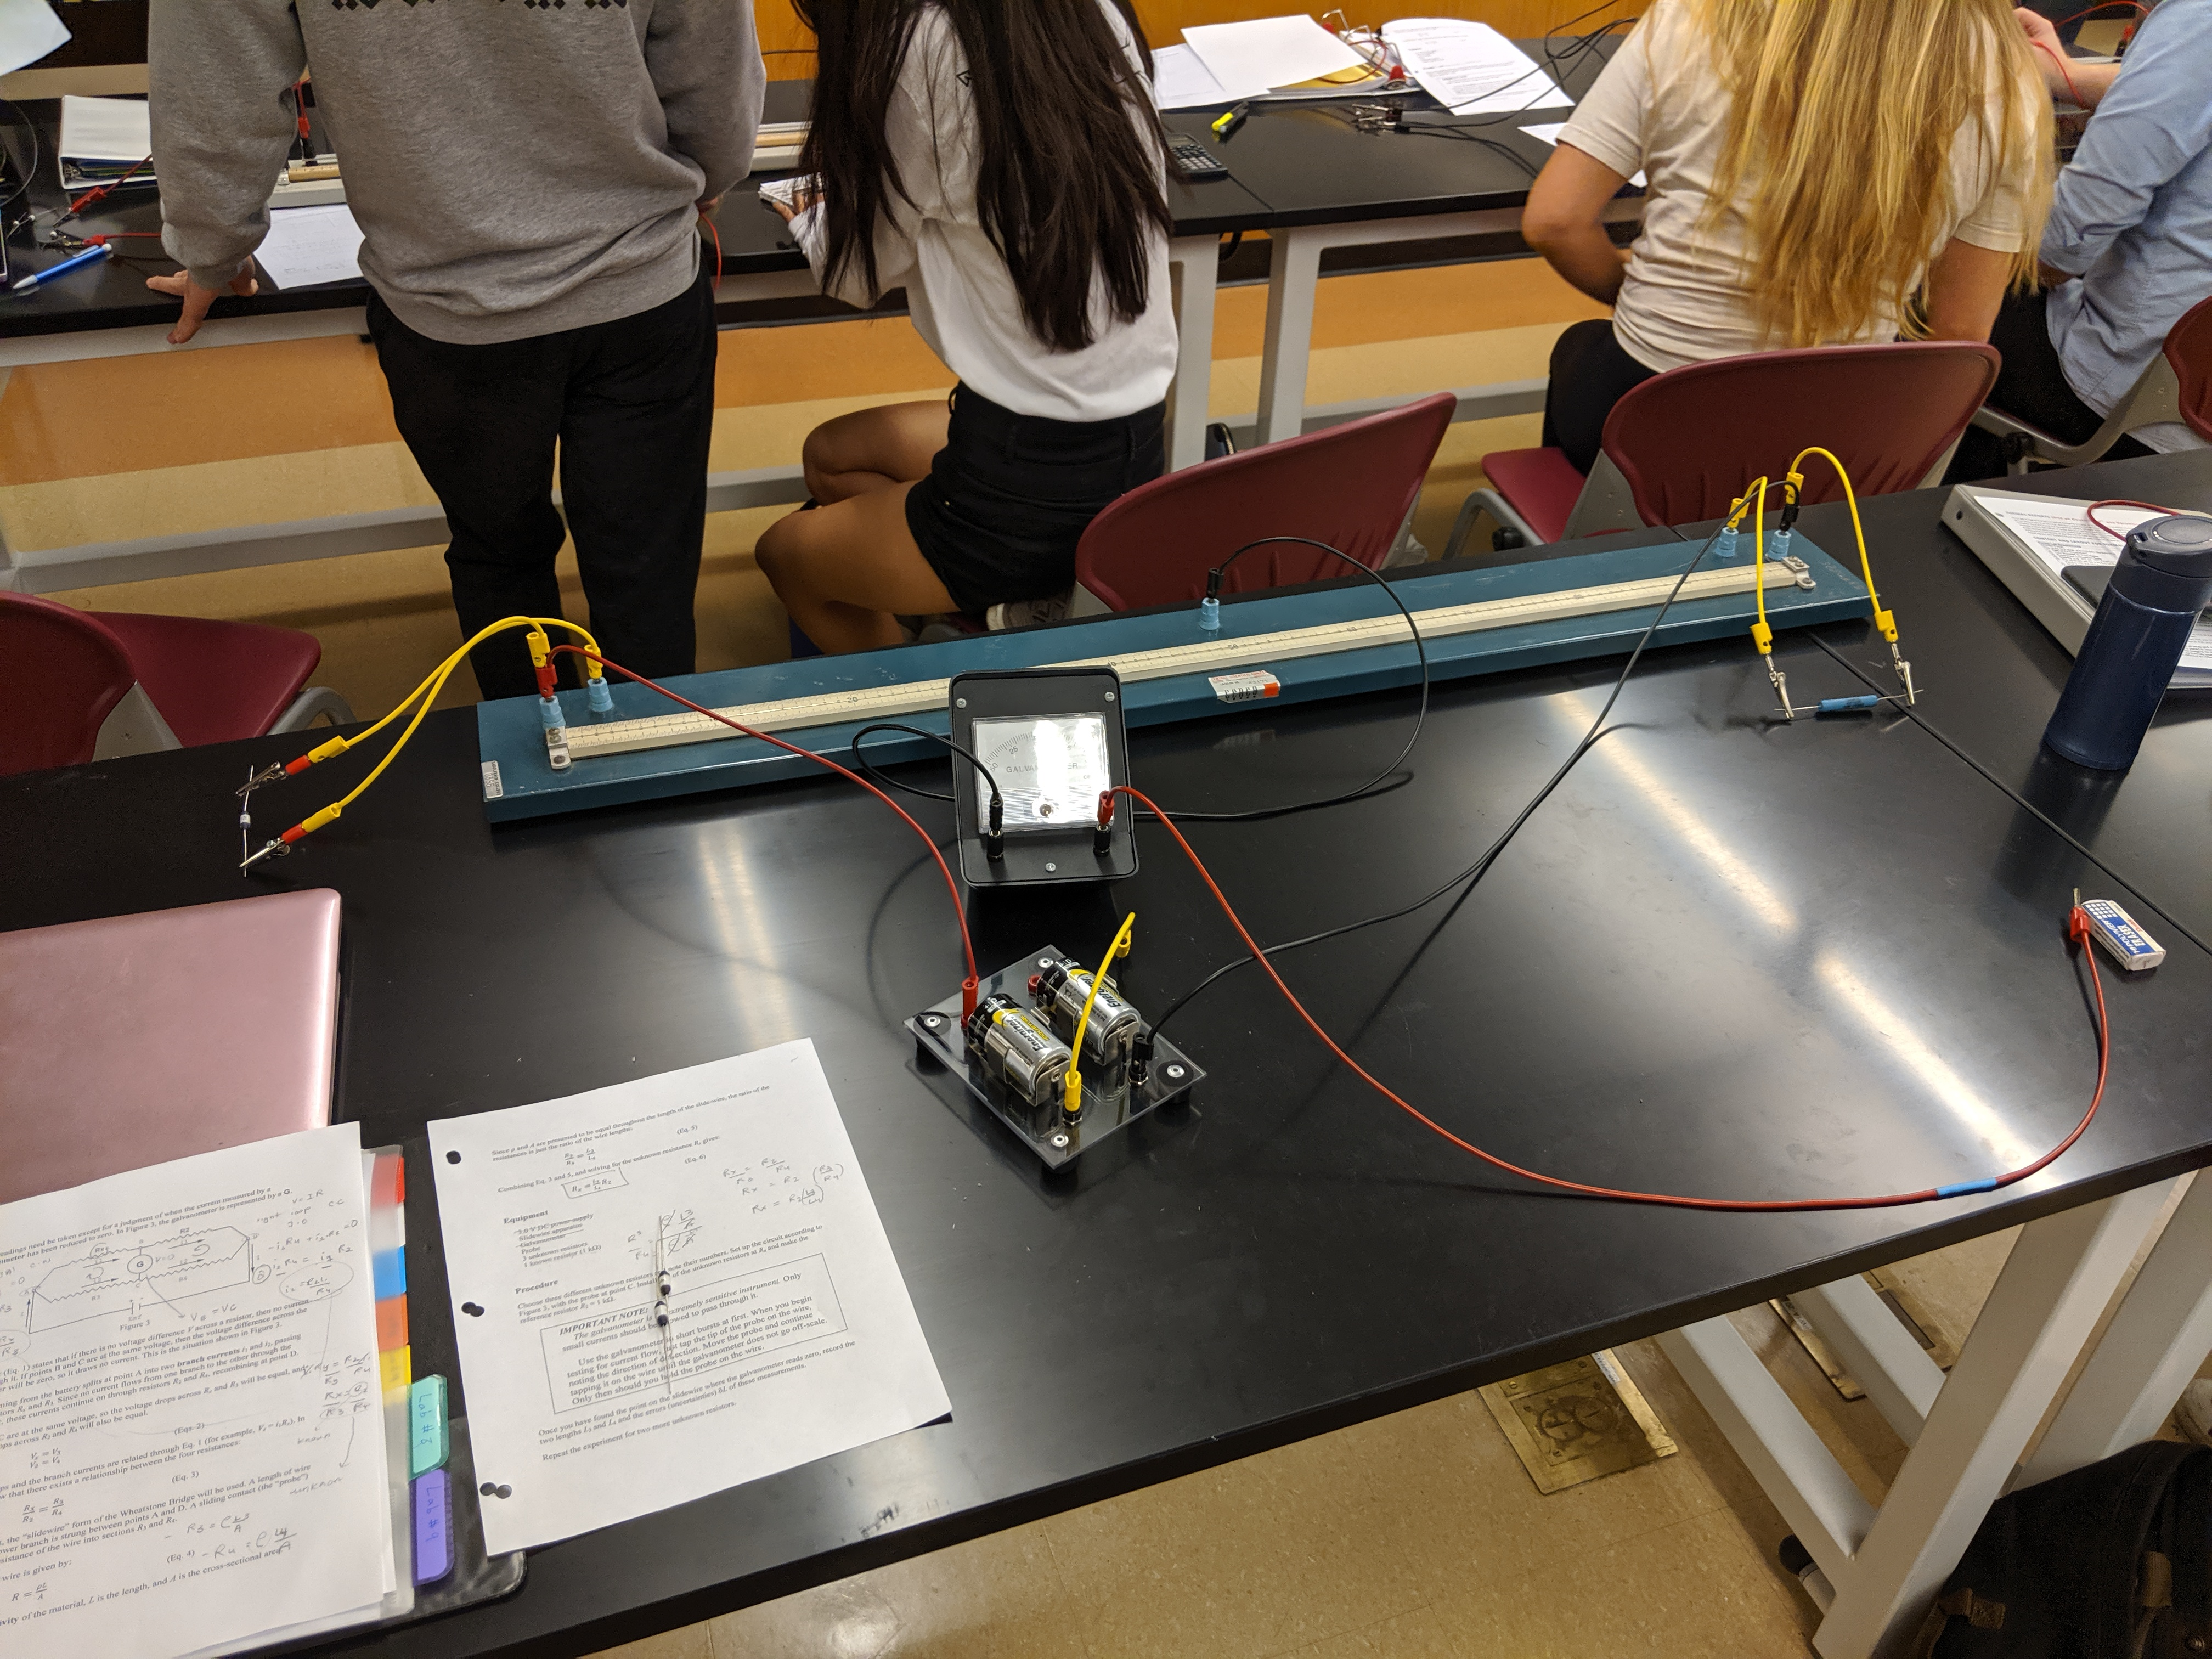
\includegraphics[width=\textwidth]{labsetup}
    \caption{Wheastone bridge setup}
    \label{fig:labsetup}
\end{figure}

\section*{Theory}

\begin{figure}[H]
    \centering
    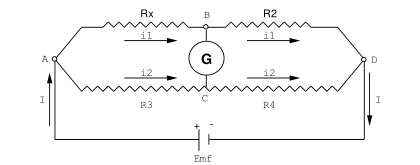
\includegraphics[width=\textwidth]{labDiagram}
    \caption{circuit diagram}
    \label{fig:diagram}
\end{figure}
\begin{table}[H]
\begin{tabular}{|l|l|}
    \hline
    \textbf{Variable}       & \textbf{Definition}                                    \\
    \hline
    V                       & Potential Difference                                   \\
    \hline
    \(V_x\)                 & Potential Difference at the unknown resistor           \\
    \hline
    \(V_2 - V_4\)           & potential difference at known resistors                \\
    \hline
    \(R_x\)                 & resistance of unknown resistor                         \\
    \hline
    \(R_x - R_4\)           & resistance of known resistors                          \\
    \hline
    \(L_3, L_4\)            & length of wire split at point of no Galvanometer reading \\
    \hline
    A                       & Amps                                                   \\
    \hline
    \(A\)                   & Area of wire                                           \\
    \hline
    \(\rho\)                & resistivity                                            \\
    \hline                                           
\end{tabular}
\end{table}

\begin{equation}
V=IR
\end{equation}
Because voltage across points B and C are the same:
\begin{equation}
V_x = V_3
V_2 = V_4
\end{equation}
Since voltage drops are related through Ohm's law (1):
\begin{equation}
\frac{R_x}{R_2} = \frac{R_3}{R_4}
\end{equation}
Resistance can be given by the following
\begin{equation}
R = \frac{\rho L}{A}
\end{equation}
Using (3) and (4) Ratio of resistances is the same as ratio of lengths:
\begin{equation}
\frac{R_3}{R_4} = \frac{L_3}{L_4}
\end{equation}
Finally using (3) and (5) and solving for unknown resistance:
\begin{equation}
R_x = \frac{L_3}{L_4}R_2
\end{equation}
\begin{equation}
\frac{|Theoretical - Experimental|}{Theoretical}100 = Percent Difference
\end{equation}

\section*{Procedure}
\begin{enumerate}
\item obtain three unknown resistors
\item construct the circuit and place unknown resistor at point \(R_x\) and known \(1000\Omega\) resistor at point \(R_2\)
\item connect the power supply and lightly tap the Galvanometer's probe alone the wire until the Galvanometer reads nothing, record this distance
\item repeat step three for the remaining unknown resistors
\end{enumerate}
\section*{Analysis}
example calculation:
\[R_x = \frac{78.5}{21.5}*1000 = 273.89\Omega\]
\[\frac{|270 - 273.89|}{270}*100 = 1.44\%\]
\subsection*{Data}
\begin{table}[H]
\csvautotabular{data.csv}
\end{table}
\section*{Conclusion}
The purpose of the experiment was met the resistances of the unknown resistors was determined experimentally and the relationships of Ohm's law held true. The percent difference between the advertised and experimental values (273.89\(\Omega\), 388.89\(\Omega\), 2703.7\(\Omega\)) was 1.44, 0.28, and 0.13 percent for the three unknown resistors. This is well within the margin of error since the tollerance for the resistors was 5\%. The change in resistance as the resistors heated up was not taken into account and could have effected the actual resistance if sufficient time was given for the resistors to increase in temperature by a measureable amount. Aditionally neither the internal resistance of the battery nor the resistances of the wires used was taken into account which could have skewed values slightly but still well within the margin of error. The Galvanometer is a very sensitive instrument therefore induced currents from radio waves or other interference may have a minimal effect on the data collected.

\section*{Extra credit}
figure redraw with Galvanometer and battery swaped
\begin{figure}[H]
    \centering
    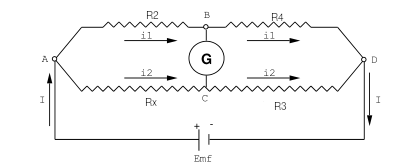
\includegraphics[width=\textwidth]{labDiagramEC}
    \caption{Extra credit}
    \label{fig:Extra credit}
\end{figure}
use kirchhoff loop rule
\begin{equation}
-R_2 i_1 + R_x i_2 = 0
\end{equation}
\begin{equation}
R_4 i_2 - R_3 i_1 = 0
\end{equation}
\begin{equation}
i_1 = \frac{R_3}{R_4}i_2
\end{equation}
\begin{equation}
i_1 = \frac{R_x}{R_2}i_2
\end{equation}
solve
\begin{equation}
\frac{R_x}{R_2} = \frac{R_3}{R_4}
\end{equation}
substitute with L3 and L4
\begin{equation}
    \frac{L3}{L4} = \frac{R3}{R4}
\end{equation}
\begin{equation}
    R_x = \frac{R_3}{R_4}R2
\end{equation}
The final equation is the same as the original
\begin{equation}
    R_x = \frac{L_3}{L_4}R2
\end{equation}
\end{document}
